\documentclass{article}

\usepackage[utf8x]{inputenc}
\usepackage[english,russian]{babel}
\usepackage{graphicx}
\usepackage{amsmath}
\usepackage{amssymb}
\usepackage{extarrows}
\usepackage{vmargin}
\usepackage{MnSymbol}
\setpapersize{A4}
\setmarginsrb{2cm}{2cm}{2cm}{2cm}{0pt}{0mm}{0pt}{13mm}
%\usepackage{cmap}

%user commands
\newtheorem{theorem}{Теорема}
\newenvironment{proof}{\paragraph{Доказательство:}}{\hfill$\blacksquare$}

\newenvironment{definition}{ \paragraph{Определение:}}{\hfill $\blacktriangleleft$}

\newenvironment{observation}{ \paragraph{Замечание:}}

\newenvironment{hence}{ \paragraph{Следствие:}}


\begin{document}

\centerline{\large Курс лекция для магистров ВМК МГУ}
\centerline {\textbf{\LARGE Обратные задачи математической физики}}
\centerline {Затехал Строков Вениамин 2025}

\vspace{0.4cm}

\centerline{\LARGE 	Лекция 9. Задача рассеяния для уравнения акустики и системы Дирака.}

\vspace{0.5cm}

Запишем систему одномерной акустики
\begin{equation*}
\begin{cases}
	\rho(y) s_t = - p_y;\\
	p_t = -\lambda(y) s_y;
\end{cases}
\quad \Leftrightarrow \quad
\rho(y)s_{tt} = (\lambda(y)s_y)_y.
\end{equation*}

где $s$ - скорость малых колебаний среды, $p$ - давление, $\rho$ - плотность, $\lambda$ - коэффициент объёмного сжатия.

Введём альтернативные коэффициенты для среды: 
$a=\sqrt{\dfrac{\lambda}{\rho}}$ - скорость распространения волны, $\sigma = a\rho$ - жёсткость (акустический импеданс).
\begin{equation*}
	s_{tt} = \dfrac{a(y)}{\sigma(y)}(a(y)\sigma(y) s_y)_y
\end{equation*}

и заменим $y$ на $x$:
\begin{equation*}
	a(y)\dfrac{d}{dy} = \dfrac{d}{dx} ,
	\quad \texttildelow \quad
	dx = \dfrac{dy}{a(y)},
	\quad \Rightarrow \quad
	x(y) = \int_0^y \dfrac{d\eta}{a(\eta)}.
\end{equation*}

$s(y(x),t) = \hat{s}(x,t)$, где $y(x)$ - функция, обратная к $x(y)$ 
\begin{equation*}
	\hat{s}_{tt} = \dfrac{1}{\hat{\sigma}(x)}(\hat{\sigma}(x) \hat{s}_x)_x = \hat{s}_{xx}+\dfrac{\hat{\sigma}'(x)}{\hat{\sigma}(x)} \hat{s}_x.
\end{equation*}

Введём новые зависимые переменные:
$\hat{v} = \hat{s}_t - \hat{s}_x$, $\hat{u} = \hat{s}_t + \hat{s}_x$,
\begin{equation*}
	(\dfrac{\partial^2}{\partial t^2} - \dfrac{\partial^2}{\partial x^2}) \hat{s} =
	(\dfrac{\partial}{\partial t} + \dfrac{\partial}{\partial x})			(\dfrac{\partial}{\partial t} - \dfrac{\partial}{\partial x}) \hat{s} =
	 \dfrac{\hat{\sigma}_x'(x)}{\hat{\sigma}(x)} \hat{s}_x;
\end{equation*}

\begin{equation*}
\begin{cases}
	(\dfrac{\partial}{\partial t} + \dfrac{\partial}{\partial x}) \hat{v} = \dfrac{\hat{\sigma}_x'(x)}{2 \hat{\sigma}(x)} (\hat{u} - \hat{v});\\
	(\dfrac{\partial}{\partial t} - \dfrac{\partial}{\partial x}) \hat{u} = \dfrac{\hat{\sigma}_x'(x)}{2 \hat{\sigma}(x)} (\hat{u} - \hat{v}).
\end{cases}
\end{equation*}

Сделаем заключительные замены:
$\hat{v} = \dfrac{v}{\sqrt{\hat{\sigma}(x)}}$,
$\hat{u} = \dfrac{u}{\sqrt{\hat{\sigma}(x)}}$, 
$z(x) = - \dfrac{\hat{\sigma}_x'(x)}{2 \hat{\sigma}(x)}$

Получим нестационарную систему Дирихле:
\begin{equation}
\begin{cases}
     v_t + v_x + z(x) u = 0;\\
     u_t - u_x - z(x) v = 0;
\end{cases}
\label{nonstatic Dirichle}
\end{equation}

где $v$ - риманов инвариант волны бегущей вправо,
$u$ - влево, $z(x)$ - коэффициент отражения (рассеяния).
\begin{equation*}
\begin{cases}
    v(x,t) = \sqrt{\hat{\sigma}(x)} (\hat{s}_t(x,t) - \hat{s}_x(x,t)),\\
    u(x,t) = \sqrt{\hat{\sigma}(x)} (\hat{s}_t(x,t) + \hat{s}_x(x,t)).
\end{cases}
\end{equation*}

и обратно
\begin{equation*}
	\begin{pmatrix}v\\u\end{pmatrix} (x,t) = 
	[\sqrt{\sigma(y)}(s_t(x,t) \mp a(y)s_y(y,t))]_{y=y(x)} 
\end{equation*}

\vspace{0.2cm}
\begin{observation}
 В систему (\ref{nonstatic Dirichle}) входит $\hat{\sigma}(x)$ и не входит $\hat{a}(x)$, поэтому возврат к переменной $y$ возможен лишь при условии задания дополнительно  $\hat{a}(x)$.
\end{observation}

\subsection*{Постановка начально-краевой задачи для системы Дирака}

Рассмотрим следующую начально-краевую задачу на полупрямой $x\geqslant 0$, $t\geqslant 0$:
\begin{equation}
\begin{cases}
    v_t + v_x + z(x) u = 0, & x,t>0;\\
    u_t - u_x - z(x) v = 0, & x,t>0;\\
    v(x,0) = v_0(x), \quad u(x,0) = u_0(x), & x >0;\\
    v(0,t) = \alpha u(0,t) + \varphi(t), & t \geqslant 0.
\end{cases}
\label{halfline system}
\end{equation}

$|\alpha| \leqslant 1$, $\varphi \in C^1$.

Пусть далее $v_0(x) = u_0(x) = 0$, $\alpha = 0$, $\varphi(0) = 0$.

\begin{definition}
Решением (\ref{halfline system}) называется пара $\{v,u\} \in C^1(\mathcal{D}) \bigcap C(\overline{\mathcal{D}})$,  $\mathcal{D} = \{x,t : x >0, t>0\}$, непрерывно примыкающая к условию на границе $\mathcal{D}$ и удовлетворяющая системе (\ref{halfline system}).
\end{definition}

\begin{observation} 
Система (\ref{nonstatic Dirichle}), (\ref{halfline system}) допускает дифференцирование по $t$. Поскольку каждое классическое решение порождает при $x>0$ обобщённую функцию, то любое решение бесконечно дифференцируемо по $t$ с соответствующими краевыми условиями.
\end{observation}


\textbf{Пример 1:} 

Пусть $v(0,t) = \dfrac{t^2}{2}$, $t\geqslant0$ ($z=0$).
Тогда $v(x,t) = \dfrac{1}{2} \tau_+^2(t-x)$, $v(x,t) = 0$, $t<0$. $u(x,t) = 0$.
Если $v(0,t) = 1 =\theta(t), t\geqslant 0$, то $v(x,t) = \theta(t-x)$, $u(x,t) = 0$.

Далее $v(0,t) = \theta'(t) = \delta(t)$, $|t|< \infty $, $v(x,t) = \theta'(t-x) = \delta(t - x)$, $u(x,t) = 0$ и т.д.

\subsection*{Задача Дарбу}

\hspace{0.2cm}
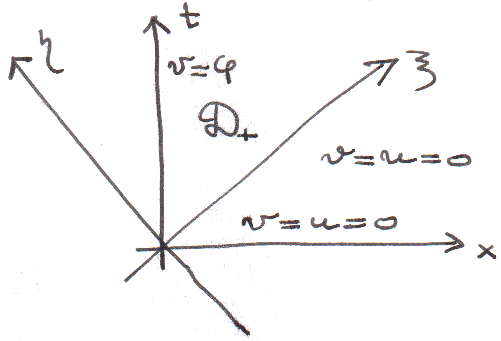
\includegraphics[scale=0.8]{pic9_1.png}
\hspace{0.2cm}

Сделаем замену $t = \xi + \eta$, $ x = \xi - \eta$, $\xi = (t+x)/2$, $\eta = (t - x)/2 \Rightarrow$
\begin{align*}
	v_{\xi} + z(\xi - \eta) u = 0, \quad & \xi + \eta > 0;\\
	u_{\eta} - z(\xi - \eta)v = 0, \quad & \xi - \eta > 0.
\end{align*}

\begin{equation*}
	t = 0: \quad
	v(\xi , -\xi) = u(\xi, - \xi) = 0, \quad \xi > 0;
\end{equation*}

\begin{equation*}
	x = 0: \quad
	v(\eta , \eta) = \varphi(\xi + \eta) =  \varphi(2 \xi) = \varphi(2 \eta).
\end{equation*}

Пусть $\varphi(t) = \theta(t)$, тогда $v(\eta, \eta) = 1$, $\eta \geqslant 0 $. 
Найдём структуру обобщённого решения.
Доказывается, что $v=u=0$ при $\eta \leqslant 0$, $u(\xi,0) = 0$ в силу непрерывности на характеристике. 
$u_{\eta}(\xi,0) = z(\xi)\theta(\xi)$, поскольку $v_{\xi}(\xi,0) = 0 \Rightarrow v(\xi,0) = \theta(\xi)$. 
Таким образом, приходим к задаче Дарбу:
\begin{equation*}
\begin{cases}
	v_t + v_x + z(x) u =0;\\
	u_t - u_x - z(x) v = 0;\\
	v(0,t) = \theta(t);\\
	u(x,x) = 0.
\end{cases}
\end{equation*}

А после дифференцирования
\begin{equation*}
\begin{cases}
	v_t + v_x + z(x) u = 0, & t > x > 0;\\
	u_t - u_x - z(x) v = 0; \\
	v(0,t) = 0, & t >0;\\
	u(x,x) = z(x) /2, & x > 0.
\end{cases}
\end{equation*}

Формально (без доказательства) это решение совпадает с обобщённым решением для (\ref{nonstatic Dirichle}) с условиями $v(0,t) = \delta(t)$, $v = u =0$ при $t<0$.

В общем случае для задачи Дарбу с условиями 
\begin{equation}
	v(0,t) = \varphi(t), \quad t>0, 
	\quad \varphi(0) = 1, \quad u(x,x) = 0,
	\label{conditions}
\end{equation}

справедлива

\begin{theorem}
Пусть $\varphi \in C^2[0,\infty)$. Тогда решение задачи Дарбу (\ref{nonstatic Dirichle}), (\ref{conditions}) $\{v,u\} \in C^1(t > x >0)$ существует, единственно и представимо в виде следующего разложения по гладкости:
\begin{equation*}
 	v(x,t) = \varphi(t-x) + V(x,t), \quad u(x,t) = U(x,t);
 \end{equation*}
где $V(x,x) = U(x,x) = 0$, $U_t(x,x) = U_x(x,x) = \dfrac{z(x)}{2}$. 
\end{theorem}
\begin{proof}
Проводится методом сведения (\ref{nonstatic Dirichle}) к системе интегральных уравнений типа Вольтерра.
Так как $u_t + u_x = 0$, рпи $t=x$, то $u_t - u_x = 2 u_t = z(x)$ при $x = t$, $u_t(x,x) = \dfrac{z(x)}{2}$.
\end{proof}

\subsection*{Оценка устойчивости}

Получим оценку устойчивости по $\varphi$, $z$.
Пусть $\varphi(t) = \varphi_1 - \varphi_2$, $z(x) = z_1 - z_2$, и $v_j(x,t) = \varphi_j(t-x) + V_j(x,t)$, $ u_j(x,t) = U_j(x,t)$, $u = u_1 -u_2$, $v = v_1 -v_2$, $U = U_1 - U_2$, $V = v_1 - V_2$:
\begin{equation*}
\begin{cases}
	V_t + V_x + z_1 U = - z U_2, & x,t>0;\\
	U_t - U_x - z_1 V = z V_2 + z_1(\varphi_1 \varphi_2;\\
	V(0,t) = 0, & t > 0;\\
	U(x,x) = 0; & x> 0.
\end{cases}
\end{equation*}

\hspace{0.2cm}
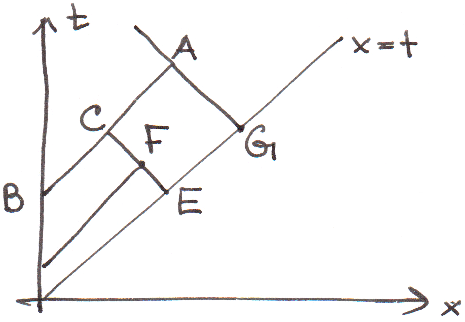
\includegraphics[scale=0.8]{pic9_2.png}
\hspace{0.2cm}

Интегрируя эту систему вдоль соответствующих характеристик получаем:
\begin{equation*}
	V(A) - V(B) - \int_{BA} z_1(c) U(c) d \xi(c) = - \int_{BA} z(c) U_2(c) d\xi(c);
\end{equation*}
\begin{equation*}
	U(c) - U(\varepsilon) = \int_{EC} z_1(F) V(F) d\tau(F) - \int_{EC} z(F) V_2(F) d\tau(F) + \int_{EC} z_1(F) (\varphi_1 - \varphi_2) (F) d\tau(F).
\end{equation*}
\begin{multline*}
	A = (x,t): \quad 
	V(x,t) = -\int_{BA} z(c) U_2(c) d\xi(c) - \int_{BA} z_1(c) U(c) d\xi(c)
	= -\int_{BA} z_1(c) U_2(c) d\xi(c) - \\
	- \int{BA} z_1(c)\int_{EC} z_1(F) V(F) d\tau_F d\xi(c) 
	- \int_{BA} z_1(c) \int_{EC} z(F) V_2(F) d\tau(F) d\xi(c) - \int_{BA} z_1(c) \int_{EC} z_1(F) \varphi(F) d\tau(F) d\xi(c).
\end{multline*}

Пусть $m(t) = \max_{x + \tau \leqslant t} |V(x,\tau)|$. Тогда:
\begin{equation*}
	m(t) \leqslant c_0 \max_{\tau \leqslant t} |\varphi(\tau)| + c_1 \int_0^t |z(\tau) d \tau + c_2 \int_0^t m(\tau) d\tau
\end{equation*}

Из леммы Гронуолла следует:
\begin{equation*}
	m(t) \leqslant const(||\varphi||_{C[0,t]}+ \int_0^t ||z||_{C[0,\tau]} d\tau).
\end{equation*}
Таким образом:
\begin{equation*}
	|V_1(x,t) - V_2(x,t)| \leqslant const(y) (||\varphi_1 - \varphi_2||_{C[0,2y]} + \int_0^y ||z_1 - z_2||_{C[0,\tau]} d \tau),
\end{equation*}

где $x+t \leqslant 2y$, $const$ зависит от $y, \varphi_1, \varphi_2, z_1, z_2$ при $t\leqslant 2y$, $z\leqslant y$.

Аналогично для производной $V_t(x,t)$ при $\varphi_1 = \varphi_2$:
\begin{equation*}
	|V_{1,t} (x,t) - V_{2,t}(x,t)| \leqslant 
	const(||\varphi_1' - \varphi_2'||_{C[0,2y]} + ||z_1 + z_2||_{C[0,y]});
\end{equation*}

где $x + t \leqslant 2y$, $const$ зависит от $\varphi_j', z_j$ при $t \leqslant 2y$, $x\leqslant y$.

\begin{hence}
Для решения задачи Дарбу (\ref{nonstatic Dirichle}),(\ref{conditions}) с условиями $v(0,t) = 0$, $u(x,x) = \dfrac{z(x)}{2}$ справедлива оценка, где $2\xi = x + t$:
\begin{equation*}
	|v(x,t)| \leqslant c_0 ||z||_{C[0,\xi]}, \quad
	|u(x,t)| \leqslant c_1 ||z||_{C[0,\xi]}.
\end{equation*}
\end{hence}

\subsection*{Единственность решения обратной задачи рассеяния для системы Дирака}

Вернёмся к задаче рассеяния для системы Дирака:
\begin{equation}
\begin{cases}
	v_t + v_x + z(x) u = 0, & x,t>0;\\
	u_t - u_x - z(x) v = 0;\\
	v(x,0) = u(x,0) = 0, & x > 0;\\
	v(0,t) = \varphi(t), & t \geqslant 0.
\end{cases}
\label{Dirak system}
\end{equation}

Поставим следующую обратную задачу на $[0,T]$:
\begin{enumerate}
\item $\varphi(t) \in C^1[0,2T]$, $\varphi(0) = q \neq 0$;
\item $f(t) \in C^1[0,2T]$, $f(0) = 0$, $ f(t) = u(0,t)$;
\end{enumerate}
найти $z(x) \in C[0,t]$.

\begin{theorem}
(Единственности)\\
Пусть выполнены условия 1) и 2) и $T > 0$. Тогда ОЗ не может иметь более одного решения $z \in C[0,T]$. Эти условия также гарантируют разрешимость в целом.
\end{theorem}
\begin{proof}
(от противного)\\
Пусть $\exists z_1 \neq z_2$. Проинтегрируем систему (\ref{Dirak system}) вдоль характеристики $x + \tau = 2t$:

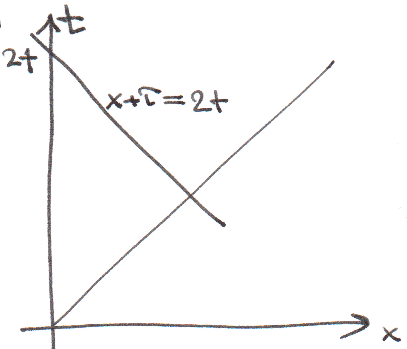
\includegraphics[scale=0.8]{pic9_3.png}

\begin{equation*}
	u_j(0,2t) - u_j(x,x) = \int_0^t v_j(x,2t - x) z_j(x) dx,
\end{equation*}

откуда

\begin{equation*}
	\int_0^t v_j(x,2t-x) z_j(x) = f(2t).
\end{equation*}

Продифференцируем это равенство, представив $v_j = \varphi(t-x) + V_j$, $\varphi(0) = q$:
\begin{equation*}
	q z_j(t) + 2 \int_0^t V_{j,t} (x,2t -x) z_j(x) dx = 2f'(2t), \quad 0\geqslant t \geqslant T.
\end{equation*}

Для $z = z_1 - z_2$ имеем:
\begin{equation*}
	q z(t) + \int_0^t V_{1,t} (x,2t-x) z(x) dx + \int_0^t V_t (x,2t-x) z_2(x) dx = 0.
\end{equation*}

Используем оценку устойчивости для $V_t$:
\begin{equation*}
	q||z||_{C[0,T]} \geqslant const \int_0^t ||z||_{C[0,\xi]} d\xi.
\end{equation*}

Из Леммы Грануолла $\Rightarrow z = 0$.
\end{proof}

\end{document} 